\documentclass[xcolor=table]{beamer}

\usetheme[secheader,compress]{Madrid} %Primary theme

\usepackage{verbatim}
\usepackage{graphicx}

%% UTM Colors
\definecolor{UTMblue}{rgb}{0.043137, 0.137254, 0.254901}
\definecolor{UTMorange}{rgb}{1.0, 0.509803, 0}

\setbeamercolor{palette primary}{bg=UTMblue,fg=white}
\setbeamercolor{palette secondary}{bg=UTMblue,fg=white}
\setbeamercolor{palette tertiary}{bg=UTMblue,fg=white}
\setbeamercolor{palette quaternary}{bg=UTMblue,fg=white}
\setbeamercolor{structure}{fg=UTMblue} % itemize, enumerate, etc
\setbeamercolor{section in toc}{fg=UTMblue} % TOC sections
\setbeamercolor{title}{fg=UTMorange}

\setbeamercolor{subsection in head/foot}{bg=UTMorange,fg=white}

%%%%%%%%%%% BEGIN MACROS %%%%%%%%%%%%%%%%%%
% frameT: Frame with title
\newcommand{\frameT}[2]{\frame{\frametitle{#1} #2}}

% frameF: Fragile frame with title
\newcommand{\frameF}[2]{
  \begin{frame}[fragile]
    \frametitle{#1}
    #2
  \end{frame}
}

% frameTop: Frame aligned t the top
\newcommand{\frameTop}[2]{\frame[t]{\frametitle{#1} #2}}


\newcommand{\tab}{\hspace{1cm}}

\newcommand{\spaceor}{\hspace{5pt} \textbf{or} \hspace{5pt}}

%%%%%%%%%%% END MACROS %%%%%%%%%%%%%%%%%%%%



\begin{document}

\title{Project Spellda}

\author{Steven Gray, James Nail, and Logan Brown}
\institute{UT-Martin}
\date{\today}

%%%%%%%%%%% BEGIN TITLE %%%%%%%%%%%%%%%%%%
\frame{\titlepage}

 %\section{Outline}
%%%%%%%%%%%% END TITLE  %%%%%%%%%%%%%%%%%%


\section{Introduction}
\frameT{Motivation} {
	\bigskip
  \begin{enumerate}
    \item Wanted to try something new to each of us
      \bigskip
    \item Wanted to do something we were all interested in
  \end{enumerate}

  \bigskip
}

\section{Goals}

\frameT{Project Goals} {
	\begin{enumerate}
		\item 3 Levels: Tutorial, Overworld, and Dungeon
		\bigskip
		\item 4-6 different enemies, 2 melee and 2-4 ranged
		\bigskip
		\item 4 different elements to control
		\bigskip
		\item Various puzzles and offshoots to incentivize exploration
	\end{enumerate}
}


\frameT{Future Direction}{
	\begin{enumerate}
		\item Narrative
		\bigskip
		\item Secret Boss(/es)
		\bigskip
		\item More dungeons and an Expanded Overworld
		\bigskip
		\item Elemental weaknesses/resistences
	\end{enumerate}
}


\section{Development}

\frameT{Engine} {
	\begin{center}
		Godot/GDScript
		\bigskip
	\end{center}
	
	\begin{center}
		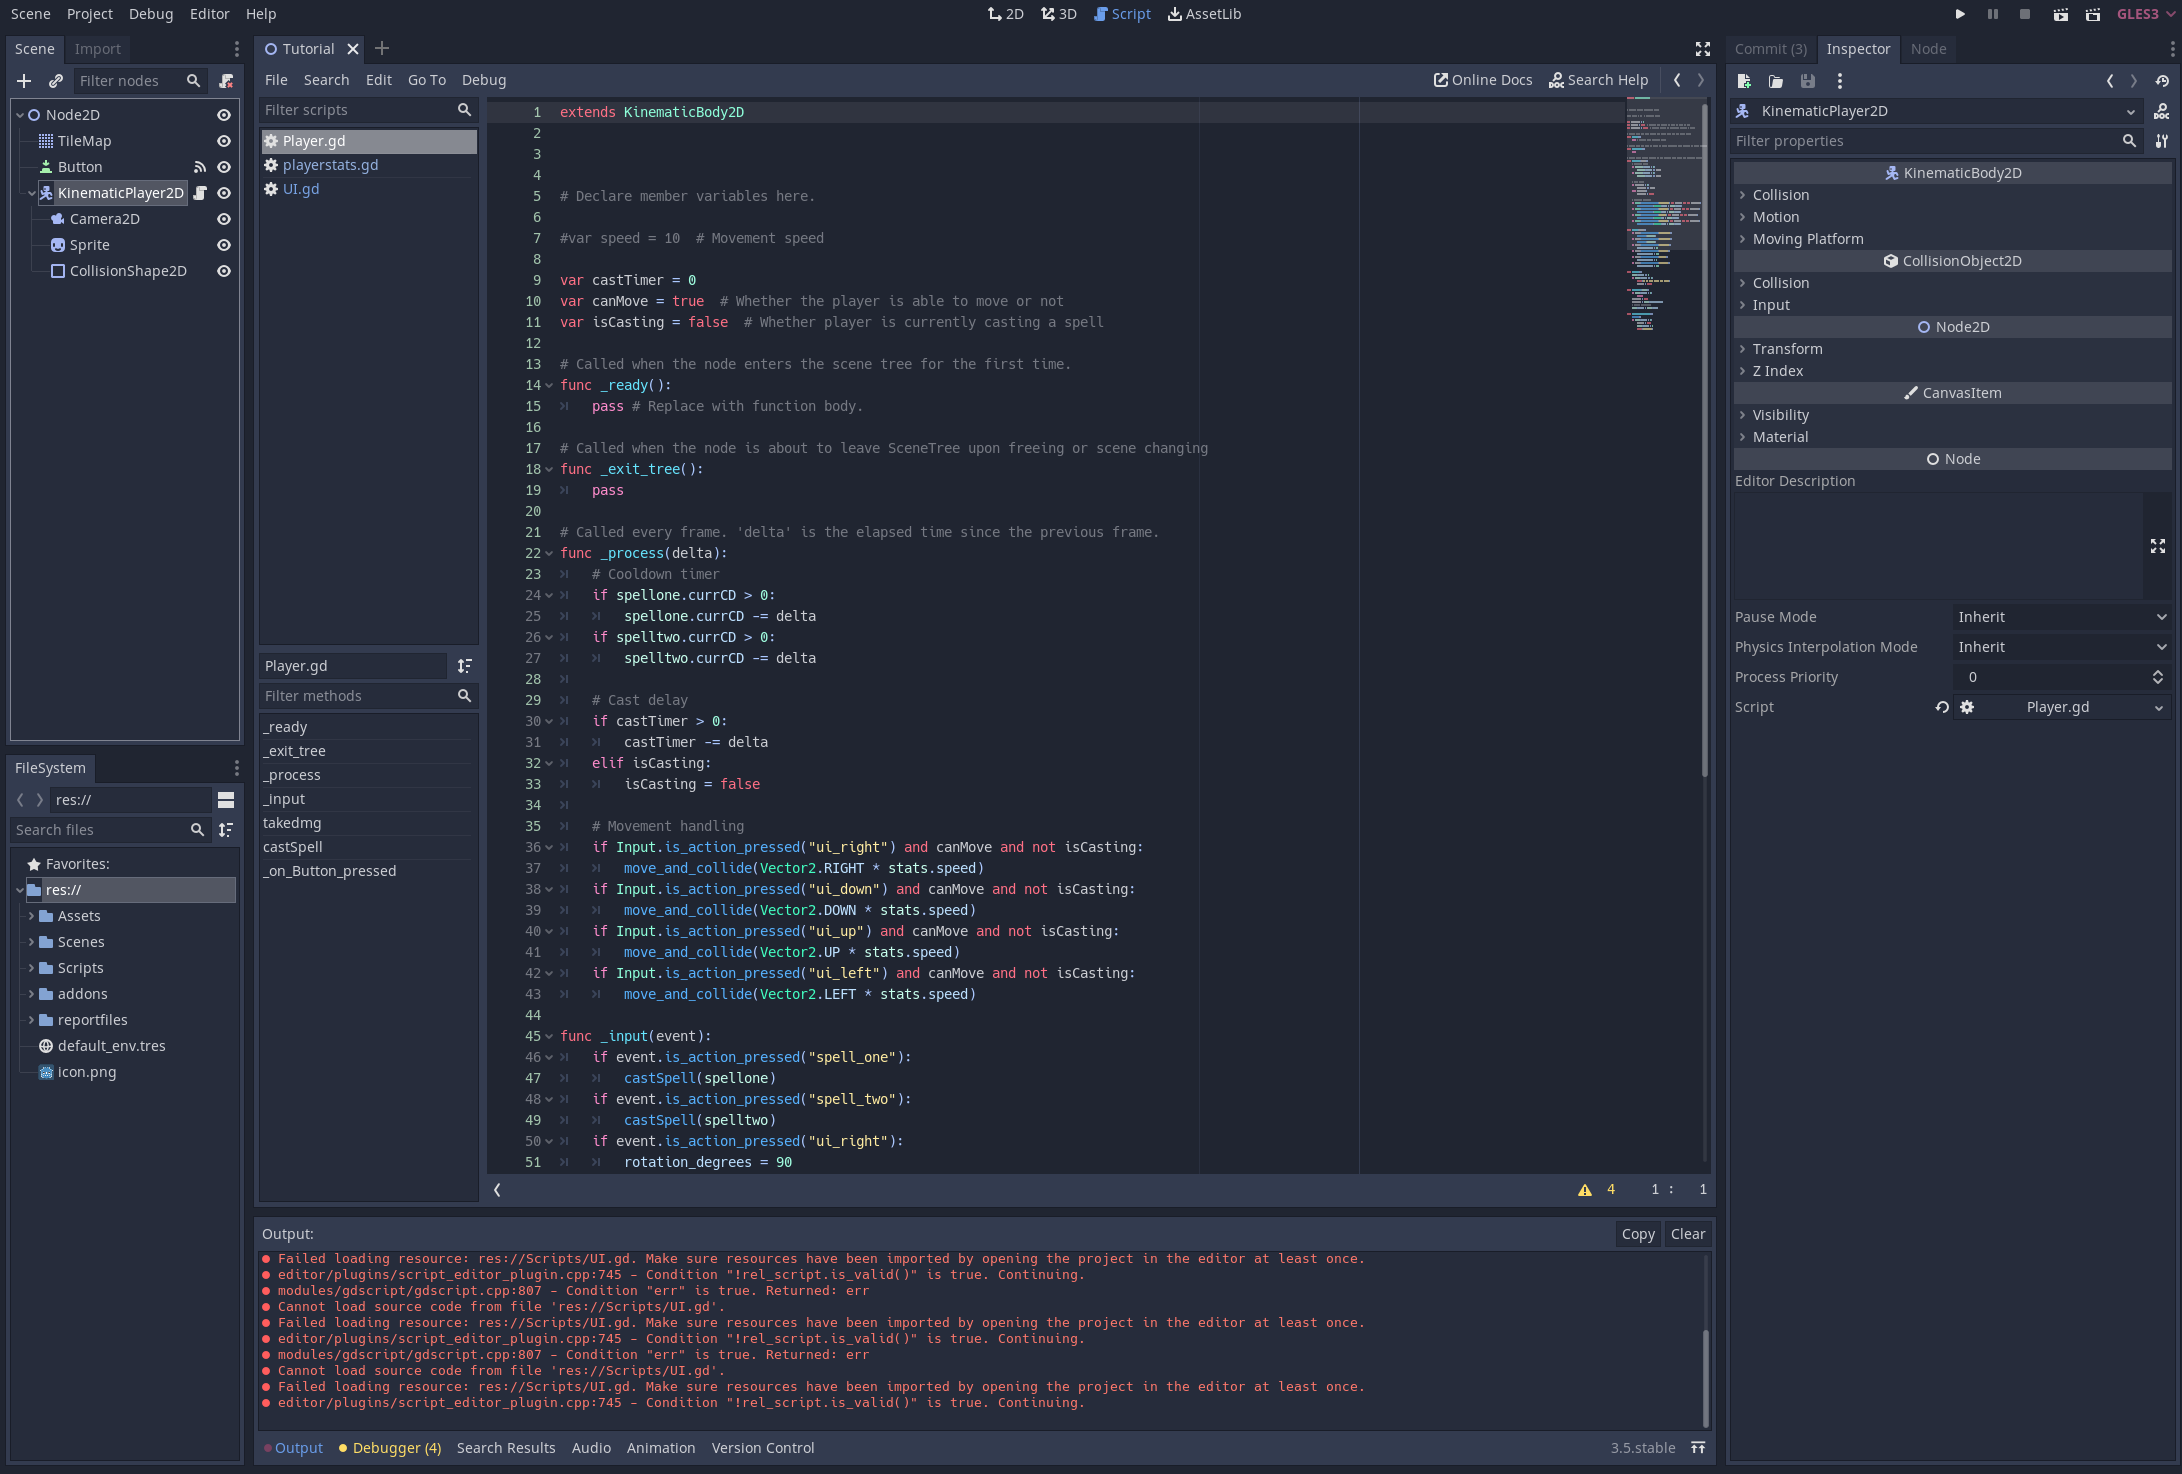
\includegraphics[width=.7\linewidth]{figures/godotscreenshot.png}
	\end{center}
}

\frameT{Inspirations} {
	\begin{figure}[ht]
    \begin{minipage}[b]{0.53\linewidth}
      \centering
			\begin{itemize}
				\item Aesthetically: Thomas was Alone/Illumine
					\bigskip
				\item Mechanically: The Legend of Zelda (NES)
			\end{itemize}
    \end{minipage}
    \hspace{0.5cm}
    \begin{minipage}[b]{0.4\linewidth}
      \centering
				%  ------- post pictures here --------
    \end{minipage}
  \end{figure}
}

\frameT{Demo} {
Here is a look into what we have!
\bigskip

\begin{center}
	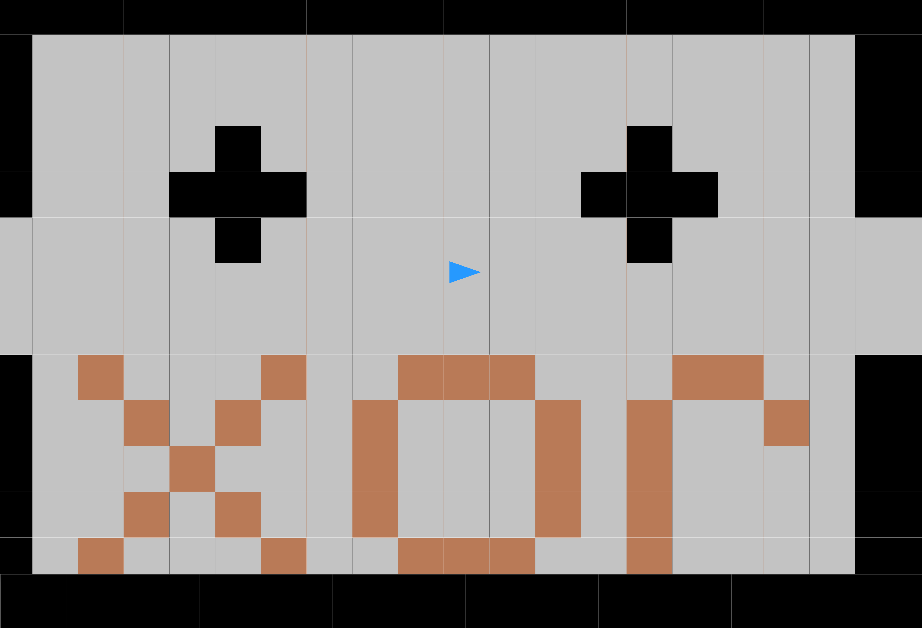
\includegraphics[width=.7\linewidth]{figures/project.png}
\end{center}
}

\frameT{Changes from Initial Design} {
	% TURN THIS INTO A COUPLE SLIDES
	Over the course of development, our focus ended up shifting
	\begin{itemize}
		\item Less spell focus
		\bigskip
		\item More focus on dungeon and puzzle design
		\bigskip
		\item More attention to lighting
	\end{itemize}
}

%\frameT{Troubles} {
	
%}

\section{Conclusion}
\frameT{Results} {
	\begin{itemize}
		\item What did we get from this project?
			\bigskip
		\item Where do we go from here?
	\end{itemize}
}

\frameT{Thank You} {
  
	\begin{center}
		Contact Us!
	\end{center}

  \begin{center}
    Questions?
  \end{center}
  
  \begin{center}
    Comments?
  \end{center}


  \bigskip
  
  \begin{center}
  Further project/author information:
  \end{center}  

  \begin{center}
    https://github.com/steagray/FA22-Senior-Design
  \end{center}

  \begin{center}
	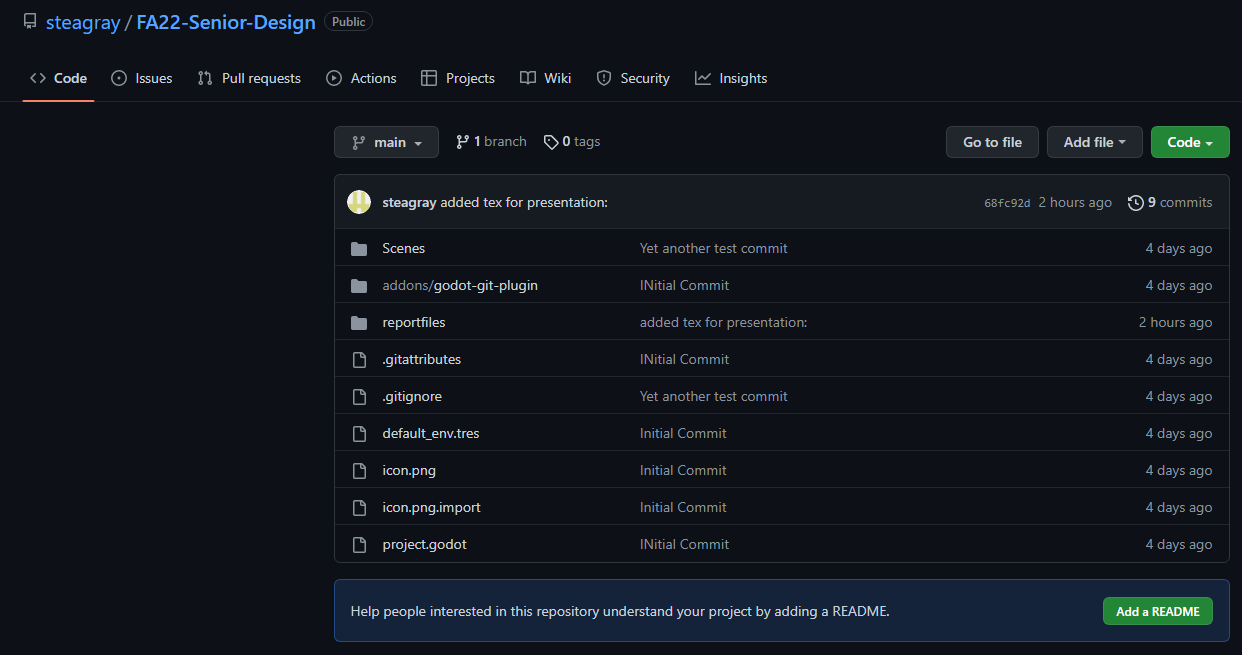
\includegraphics[width=10cm]{figures/gitpage.png}
  \end{center}
}

%\frameF{fragile test} {
%}

%% \frameF{Prolog Family Tree} {
%% \begin{verbatim}
%% hello
%% \end{verbatim}



%% }

%Empty Page
%\frameT{Frame 1}{
%}  


\end{document}
